\chapter{Non-communication Hardware Functions}

In addition to communication buses, described in chapter~\ref{ch:hw_buses}, GEX implements several measurement and output functions that take advantage of the microcontroller's peripheral blocks, such as timers/counters and \gls{DAC}. The more complicated ones are described here; simpler functions, such as the raw \gls{GPIO} access, will be described later together with their control \gls{API}.

\section{Frequency Measurement} \label{sec:theory-fcap}

Applications like motor speed measurement and the reading of a \gls{VCO} or \gls{VCO}-based sensor's output demand a tool capable of measuring frequency. This can be done using a laboratory instrument such as the Agilent 53131A. A low-cost solution can be realized using a timer/counter peripheral of a microcontroller.

\noindent
Two basic methods to measure frequency exist~\cite{fcap-twotypes}, each with its advantages and drawbacks:

\begin{itemize}
	\item The \textit{direct method} (fig.~\ref{fig:fcap-direct-dia}) is based on the definition of frequency as a number of cycles $n$ in a fixed-length time window $\tau$ (usually 1\,s); the frequency is then calculated as $f=n/\tau$.

	One timer generates the time window and its output gates the input of another, configured as a pulse counter. At the end of the measurement window an interrupt is generated and we can read the pulse count from the counter's register.

	The direct method has a resolution of 1\,Hz with a sampling window of 1\,s (only a whole number of pulses can me counted). The resolution can be increased by using a longer time window, provided the measured signal is stable enough to make averaging possible without distorting the result. Further increase of precision is possible through analog or digital interpolation~\cite{fcap-increasing}, a method used in some professional equipment.

	\item The \textit{indirect} or \textit{reciprocal method} (fig.~\ref{fig:fcap-reci-dia}) measures one period $T$ as the time interval between two pulses and this is then converted to frequency as $f=1/T$.

	This method needs only one timer/counter. Cycles of the system clock are counted for the duration of one period on the input pin (between two rising edges). If we additionally detect the falling edge in between, the counter's value gives us the duty cycle when related to the overall period length.

	Te reciprocal method's resolution depends on the counter's clock speed; if driven at 48\,MHz, the tick period is 20.83\,ns, which defines the granularity of our time measurement. It is common to measure several pulses and average the obtained values to further increase the precision.

	We can easily achieve a sub-hertz resolution with this method, but its performance degrades at high frequencies where the time measurement precision becomes insufficient. The input frequency range can be extended using a hardware prescaller\footnote{\textit{Prescaller} is a divider implemented as part of the timer/counter peripheral block that can be optionally enabled and configured to a desired division factor.}, which is also applicable to the direct method, should the measurement of frequencies outside the counter's supported range be required. A duty cycle measurement available in this method can be used to read the output of sensors that use a pulse-width modulation.

\end{itemize}

\begin{figure}[h]
	\centering
	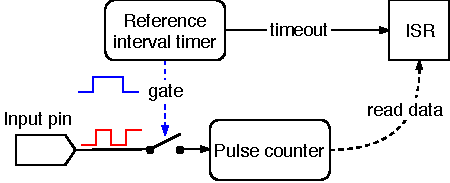
\includegraphics[scale=1] {img/fcap-direct.pdf}
	\caption{\label{fig:fcap-direct-dia}Direct frequency measurement method}
\end{figure}

\begin{figure}[h]
\centering
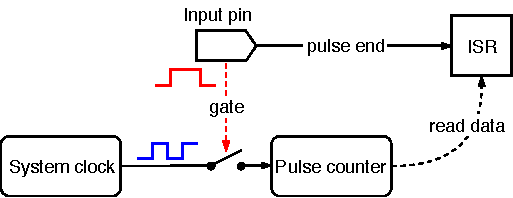
\includegraphics[scale=1] {img/fcap-reciprocal.pdf}
\caption{\label{fig:fcap-reci-dia}Reciprocal frequency measurement method}
\end{figure}

Which method to use depends on the frequency we want to measure; the worst-case measurement errors of both methods, assuming an ideal 48\,MHz system clock, are plotted in figure~\ref{fig:freqmethods-graph}. It can be seen that the reciprocal method leads in performance up to 7\,kHz where the direct method overtakes it. If a higher error is acceptable, the reciprocal method could be used also for higher frequencies to avoid a reconfiguration and to take advantage of its higher speed.

\begin{figure}[h]
	\centering
	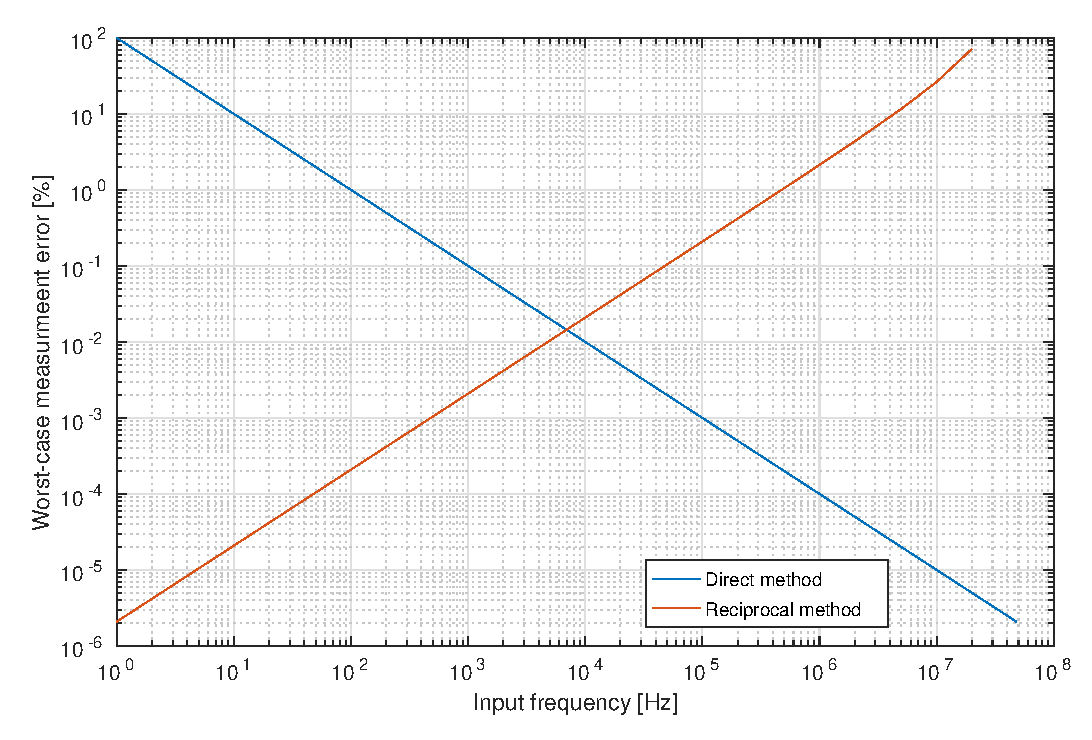
\includegraphics[width=\textwidth] {img/freqmethods.eps}
	\caption[Frequency measurement methods comparison]{\label{fig:freqmethods-graph}Worst-case error using the two frequency measurement methods with an ideal 48\,MHz timer clock. The crossing lies at 7\,kHz with an error of 0.015\,\%, or 1.05\,Hz.}
\end{figure}

A good approach to a universal measurement, for cases where we do not know the expected frequency beforehand, could be to obtain an estimate using the direct method first, and if the frequency is below the worst-case error crossing point (here 7\,kHz, according to figure~\ref{fig:freqmethods-graph}), to take a more precise measurement using the reciprocal method.

The system clock's frequency, which we use to measure pulse lengths and to gate the pulse counter, will be affected by tolerances of the used components, the layout of the \gls{PCB}, temperature effects etc., causing measurement errors. A higher accuracy could be achieved using a \gls{TCO}, or, in the direct method, with the synchronization pulse provided by a \gls{GPS} receiver to time the measurement interval.

\section{Analog Signal Acquisition} \label{sec:theory-adc}

A very common need in experiments involving the measurement of physical properties is the acquisition of analog signals, respective voltages. Those can be roughly divided into \gls{DC} and \gls{AC} or time-changing signals. Analog signals are converted to digital values using \glspl{ADC}. Several principles of analog signal measurement exist with different cost, speed, resolution, and many other factors which determine their suitability for a particular application.

\gls{DC} signals can be measured by taking several samples and calculating their average value; in the presence of a 50\,Hz or 60\,Hz mains interference, its advisable to spread those samples over the 20\,ms (resp. 16.7\,ms) time of one period so that the interfering waveform cancels out. Time-changing signals can be captured by taking isochronous samples at a frequency conforming to the Nyquist theorem, that is, at least twice that of the measured signal. In practice, a frequency several times higher is preferred for a more accurate capture.

\begin{figure}
	\centering
	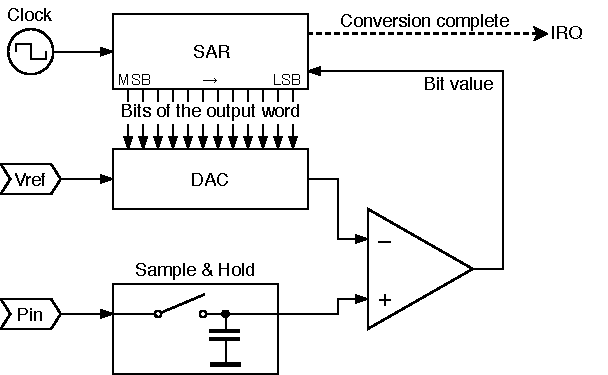
\includegraphics[scale=1] {img/sar-adc.pdf}
	\caption{\label{fig:adc-sar}A diagram of the SAR type ADC}
\end{figure}

The \gls{ADC} type commonly available in microcontrollers, including our STM32F072, uses a \textit{successive approximation} method. It is called the \textit{SAR type \gls{ADC}}, after its main component, the \gls{SAR}. A diagram of this \gls{ADC} is shown in figure~\ref{fig:adc-sar}.

The \gls{SAR} type converter uses a \gls{DAC}, controlled by the value in the \gls{SAR}, which approximates the input voltage, bit by bit, following the algorithm described in~\cite{adc-sar} and outlined below:

\begin{enumerate}
	\item The \gls{SAR} is cleared to all zeros.
	\item The \gls{DAC} generates an approximation voltage.
	\item Its output is compared with the sampled input, and the comparator's output is stored as the active bit in the approximation register.
	\item The approximation continues with step 2 and the following (less significant) bit.
	\item When all bits of the data word were found, an interrupt request is generated and the application program can read it from the \gls{SAR}.
\end{enumerate}

A change of the input value would make this principle unreliable, which is why the input is buffered by a sample \& hold circuit. The holding capacitor is charged to the input voltage and maintains this level during the conversion. The duration for which the capacitor is connected to the input is called a \textit{sampling time}.

\section{Waveform Generation} \label{sec:theory-dac}

A waveform generator is a useful tool in many experiments and measurements. A sine stimulus is the basis of a lock-in amplifier; it can be used to measure impedance; with a frequency sweep, we can obtain the frequency response of an analog filter, etc. We can, of course, generate other waveforms, such as a triangle, ramp, or rectangle wave.

The \gls{DAC} peripheral can produce a \gls{DC} level on the output pin based on a control word. When we periodically change its digital input, it produces an analog waveform.

\subsection{Waveform Generation with DMA and a Timer} \label{sec:theory-dac-simple}

A straightforward, intuitive implementation of the waveform generator is illustrated in figure~\ref{fig:wavegen-naive}. This approach has its advantages: it is simple and works autonomously, with no interrupt handling or interventions from the program. It could be implemented without the use of \gls{DMA} as well, using a loop periodically updating the \gls{DAC} values; of course, such approach is less flexible and we would run into problems with interrupt handling affecting the timing accuracy.

\begin{figure}[h]
	\centering
	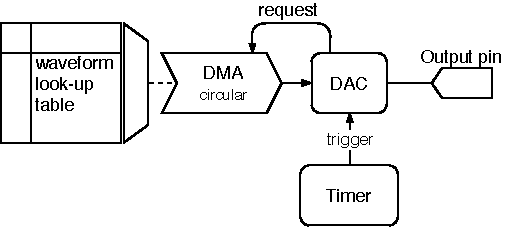
\includegraphics[scale=1.1] {img/wavegen-naive.pdf}
	\caption[A simple implementation of the waveform generator]{\label{fig:wavegen-naive}A simple implementation of the waveform generator, using DMA and a look-up table}
\end{figure}

The highest achievable output frequency largely depends on the size of our look-up table. For instance, assuming a timer frequency of 48\,MHz and a 8192-word table, holding one period of the waveform, the maximum frequency would be short of 6\,kHz, whereas if we shorten the table to just 1024 words, we can get almost 47\,kHz on the analog output. The downside of a shorter table is a lower resolution, which will appear as \gls{DC} plateaus or steps when observed with an oscilloscope, producing harmonic components similar to those of a square wave.

A major disadvantage of this simple generation method is given by the limitations of the used timer, which defines the output frequency. Its output trigger fires when the internal counter reaches a pre-defined value, after which the counting register is reset. The counting speed is derived from the system clock frequency $f_\mathrm{c}$ using a prescaller $P$ and the set maximum value $N$. Only output frequencies that can be exactly expressed as $f=f_\mathrm{c}/(P\cdot N \cdot \mathrm{TableSize})$ can be accurately produced. Still, this simple and efficient method may be used where fine tuning is not required to take advantage of its fully asynchronous operation.

\subsection{Direct Digital Synthesis} \label{sec:theory-dac-dds}

There are situations where the simple waveform generation method is not sufficient, particularly when a fine tuning or on-line frequency and phase changes are required. Those are the strengths of \gls{DDS}, an advanced digital waveform generation method well explained in~\cite{all-about-dds}.

\begin{figure}[h]
	\centering
	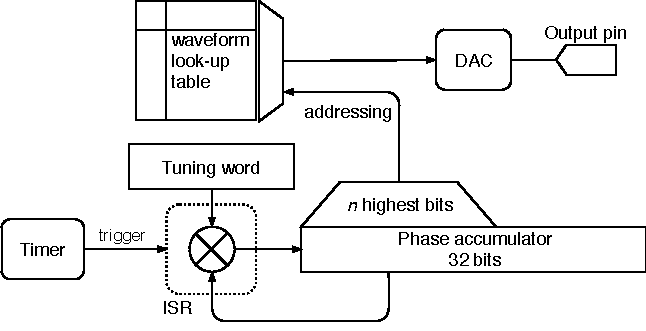
\includegraphics[scale=1] {img/wavegen-dds.pdf}
	\caption{\label{fig:wavegen-dds}A block diagram of a DDS-based waveform generator}
\end{figure}

A diagram of a possible \gls{DDS} implementation in the STM32 firmware is shown in figure~\ref{fig:wavegen-dds}. It is based on a \gls{NCO}. The \gls{NCO} consists of a \textit{phase accumulator} register and a \textit{tuning word} which is periodically added to it at a constant rate in a timer interrupt handler. The value of the tuning word determines the output waveform frequency. The look-up table must have a power-of-two length so that it can be addressed by the \textit{n} most significant bits of the phase accumulator. An additional control word could be added to this address to implement a phase offset for applications like a phase-shift modulation.

The output frequency is calculated as \(f_\mathrm{out} = \dfrac{M\cdot f_\mathrm{c}}{2^n}\), where $M$ is the tuning word, $n$ is the bit length of the phase accumulator, and $f_c$ is the frequency of the phase-updating interrupt. The number of bits used to address the look-up table does not affect the output frequency; the table can be as large as the storage space allows. A tuning word value exceeding the lower part of the phase accumulator (including bits which directly enter the look-up address) will cause some values from the table to be skipped. A smaller tuning word, conversely, makes some values appear on the output more than once. This can be observed as steps or flat areas on the output. When the tuning word does not evenly divide $2^n$, that is, the modulo is non-zero, we can also observe jitter.

\subsubsection{DDS Implemented in Hardware}

DDS may be implemented in hardware, including the look-up table, often together with the \gls{DAC} itself, which is then called a \textit{Complete \gls{DDS}}. That is the case of e.g. AD9833 from Analog Devices. As the software implementation depends on a periodic interrupt, it is often advantageous to use a component like this when we need higher output frequencies where the use of an interrupt is not possible. GEX can control an external waveform generator like the AD9833 using an \gls{SPI} port.

\section{Touch Sensing} \label{sec:theory-touch}

The used microcontroller, STM32F072, includes a \gls{TSC} peripheral block. It can be accessed from GEX as a demonstration of capacitive touch sensing, and could possibly be used for simple touch sensors as well, such as measuring the level of water in a tank.

The TSC requires a specific topology with a sampling capacitor connected close to the microcontroller pin, which may not be possible on a universal GEX module; for this reason, the touch sensing feature is best demonstrated on the STM32F072 Discovery development kit, which includes a 4-segment touch slider shown in figure~\ref{fig:disco-touch}.

\begin{figure}[h]
	\centering
	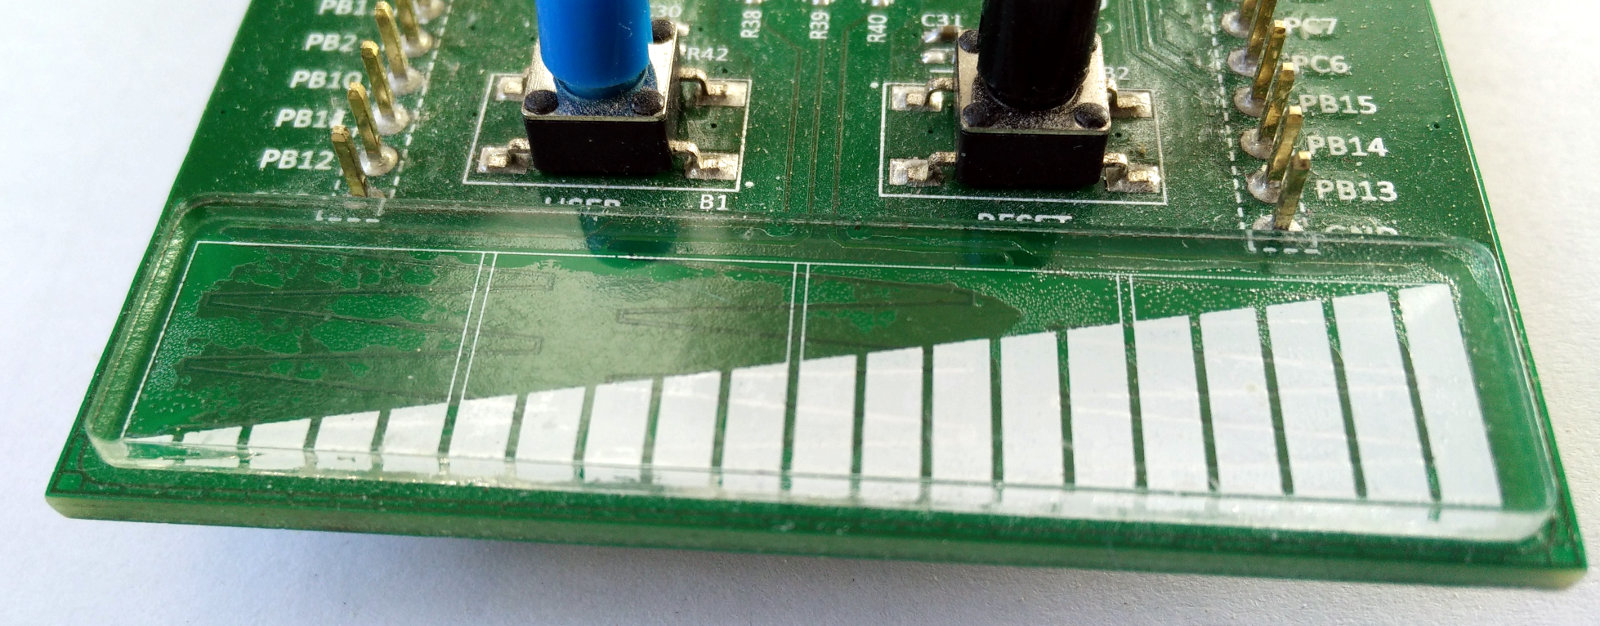
\includegraphics[width=0.5\textwidth] {img/disco-touch.jpg}
	\caption{\label{fig:disco-touch}The touch slider on a STM32F072 Discovery board}
\end{figure}

The principle of capacitive touch sensing using the \gls{TSC} is well explained in the microcontroller's reference manual~\cite{f072-rm}, the \gls{TSC} product training materials~\cite{stm-tsc-training, stm-tsc-ppt} and application notes from ST Microelectronics~\cite{stm-tsc-an1, stm-tsc-an2, stm-tsc-an3, stm-tsc-an4}. A key part of the \gls{TSC} is a set of analog switches which can be combined to form several different signal paths between external pins, Vdd, \gls{GND}, and an analog comparator. Two input pins are needed for every touch sensing channel: the sensing pad connects to one, the other is connected through a sampling capacitor  (47\,nF on the Discovery board) to \gls{GND}.

\begin{figure}[h]
	\centering
	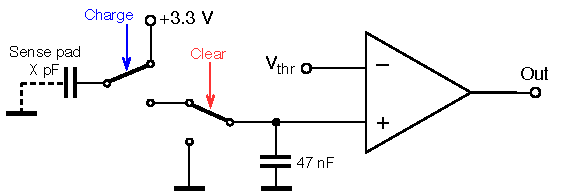
\includegraphics[scale=1] {img/tsc-function.pdf}
	\caption{\label{fig:tsc-schem}A simplified schematic of the touch sensing circuit}
\end{figure}

\noindent
Capacitive sensing is a sequential process described in the following steps:

\begin{enumerate}
	\item The sampling capacitor is discharged by connecting its free end to \gls{GND}.
	\item The sensing pad is connected to +3.3\,V and, acting as a capacitor, charged to this voltage. It stores a small amount of charge, depending on its capacitance---this is the variable property we are trying to measure.
	\item The free terminals of the two capacitors (the sensing pad and the sampling capacitor) are connected together and their voltages reach an equilibrium as a portion of the stored charge leaves the sensing pad and flows into the bigger capacitor.
	\item The steps (2) and (3) are repeated until the sampling capacitor's voltage exceeds a fixed threshold (set to a half of the supply voltage). The number of cycles needed to charge the sampling capacitor corresponds to the capacitance of the sensing pad.
\end{enumerate}

\noindent
A real voltage waveform measured on the sensing pad using an oscilloscope is shown in figure~\ref{fig:tsc-wfm}.

\begin{figure}
	\centering
	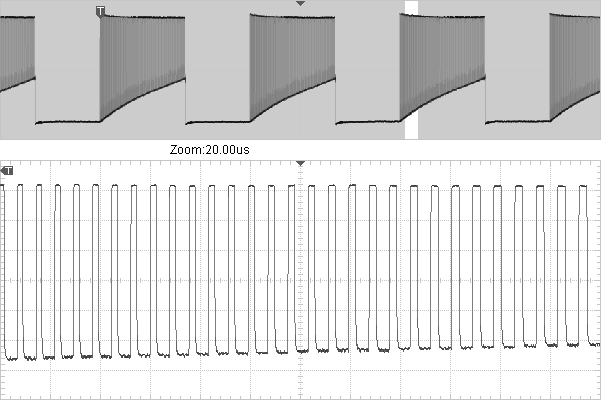
\includegraphics[width=.9\textwidth] {img/tsc-wfm-bw.png} \\
	\vspace{5mm}
	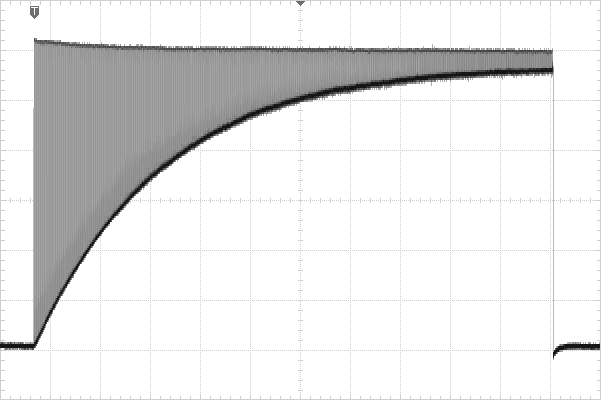
\includegraphics[width=.9\textwidth] {img/tsc-wfm2-bw.png}
	\caption[TSC operation oscilloscope screenshots]{\label{fig:tsc-wfm}A voltage waveform measured on the touch sensing pad. The bottom side of the envelope equals the sampling capacitor's voltage---this is the phase where both capacitors are connected. The detailed view (middle) shows the individual charging cycles. The bottom screenshot captures the entire waveform, left to continue until a timeout, after the analog comparator was disabled.}
\end{figure}


